\chapter{Phenotype Prediction on Synthetic Genomic Data}
\label{ch:application}

This chapter evaluates the phenotype prediction performance of SNPbag against LDpred2-auto \citep{Prive2020}. Both methods are applied to synthetic genotype data from the HAPNEST project \citep{Wharrie2023}, with phenotypes simulated under a logistic disease model. \autoref{sec:app_data} describes the data. \autoref{sec:app_pheno_sim} describes how the phenotypes are simulated. \autoref{sec:app_ldpred2} describes how LDpred2-auto is applied. \autoref{sec:app_pretrain} describes the pre-training of SNPbag. \autoref{sec:app_finetune} describes the fine-tuning of SNPbag for phenotype prediction. Finally, \autoref{sec:app_comparison} compares the two methods.

\section{Synthetic Genotype Data}
\label{sec:app_data}

The genotype data is a synthetic dataset generated by the HAPNEST framework \citep{Wharrie2023}. HAPNEST produces individual-level genotype data by resampling phased haplotypes from reference panels (the 1000 Genomes Project and the Human Genome Diversity Project), preserving realistic linkage disequilibrium patterns and allele frequency spectra \citep{Wharrie2023}.

The dataset comprises $N = 100000$ synthetic individuals. For computational feasibility, only the first $M = 14000$ SNPs on chromosome 22 are used. The genotype data is stored in PLINK binary format (.bed, .bim, .fam), and each entry of the genotype matrix $G \in \{0, 1, 2\}^{N \times M}$ encodes the minor allele count at the corresponding locus.

The $N = 100000$ individuals are split into three non-overlapping subsets: a training set of $|\mathcal{I}_{\mathrm{train}}| = 70000$ individuals ($70\%$), a validation set of $|\mathcal{I}_{\mathrm{val}}| = 10000$ individuals ($10\%$), and a test set of $|\mathcal{I}_{\mathrm{test}}| = 20000$ individuals ($20\%$). This split is shared between SNPbag and LDpred2-auto so that both methods are trained and evaluated on the same individuals.

\section{Phenotype Simulation}
\label{sec:app_pheno_sim}
The phenotype is simulated directly on the $M = 14000$ SNPs from chromosome
22 because the heritability captured by this small subset is insufficient
for either method to learn from the phenotypes distributed with the HAPNEST
dataset. The simulation uses a logistic disease model based on
\citet{Majumdar2018}. The original model generates disease status from a
single SNP with uniformly distributed odds ratios. Here, the model is
extended to a polygenic setting: $|\mathcal{M}_c| = 500$ causal SNPs
contribute simultaneously, and their log odds ratios are drawn from
$\mathcal{N}(0, \sigma_\beta^2)$ rather than a uniform distribution. The
logistic link and the calibration of the intercept to match a target
prevalence are unchanged.

\subsection{Causal SNPs and Effect Sizes}

A set of causal SNPs $\mathcal{M}_c \subset \{1, \dots, M\}$ with $|\mathcal{M}_c| = 500$ is sampled uniformly at random from the $M = 14000$ available SNPs. For each causal SNP $m \in \mathcal{M}_c$, a log odds ratio is drawn independently from a normal distribution
\begin{align*}
    \beta_m \sim \mathcal{N}(0, \sigma_\beta^2), \quad m \in \mathcal{M}_c,
\end{align*}
with $\sigma_\beta = 0.5$. The remaining $M - |\mathcal{M}_c|$ non-causal SNPs are assigned $\beta_m = 0$.

\subsection{Logistic Disease Model}

For individual $i$, the genetic component of the linear predictor is
\begin{align*}
    \eta_i^{\text{gen}} = \sum_{m \in \mathcal{M}_c} G_{i,m}\,\beta_m,
\end{align*}
where $G_{i,m} \in \{0, 1, 2\}$ is the minor allele count of individual $i$ at SNP $m$. The probability that individual $i$ is a case is given by the logistic model
\begin{align*}
    \mathbb{P}(y_i = 1 \mid G_i) = \frac{1}{1 + \exp\left(-(\alpha + \eta_i^{\text{gen}})\right)},
\end{align*}
where $\alpha$ is an intercept calibrated so that the overall population prevalence matches the target $K = 0.10$, i.e.\
\begin{align*}
    \frac{1}{N}\sum_{i=1}^{N} \frac{1}{1 + \exp(-(\alpha + \eta_i^{\text{gen}}))} = K.
\end{align*}
The intercept $\alpha$ is found by univariate root-finding. The binary phenotype is then drawn as $y_i \sim \text{Bernoulli}\!\left(\mathbb{P}(y_i = 1 \mid G_i)\right)$, producing approximately $10000$ cases and $90000$ controls.

The simulation outputs the binary phenotype $(y_1, \dots, y_N) \in \{0, 1\}^N$ and the ground-truth log odds ratios for the causal SNPs.

\section{LDpred2-auto for Phenotype Prediction}
\label{sec:app_ldpred2}

LDpred2-auto operates on GWAS summary statistics and an LD correlation matrix, as described in \autoref{sec:ldpred2}. Its application to the simulated phenotype involves three steps: running a GWAS on the training set, computing the LD correlation matrix, and running the LDpred2-auto Gibbs sampler.

\subsection{GWAS on the Training Set}

A GWAS is performed on $\mathcal{I}_{\text{train}}$ using PLINK2 \citep{Chang2015}. For each of the $M = 14000$ SNPs, a logistic regression of the binary phenotype $y_i \in \{0, 1\}$ on the genotype $G_{i,m}$ is fitted without covariates, using the Firth-corrected logistic regression implemented in PLINK2. This produces an odds ratio, a log odds ratio standard error, and a $p$-value for each SNP. The log odds ratios are used as the marginal effect estimates $\hat{\beta}_m$ in the LDpred2 pipeline. The GWAS is performed exclusively on the training set to avoid information leakage into the summary statistics.

The effective sample size for the binary trait is computed as
\begin{align*}
    N_{\text{eff}} = \frac{4}{1/n_{\text{case}} + 1/n_{\text{ctrl}}},
\end{align*}
where $n_{\text{case}}$ and $n_{\text{ctrl}}$ are the number of cases and controls in the training set.

\subsection{LD Correlation Matrix}

The LD correlation matrix $R \in \mathbb{R}^{M' \times M'}$ is computed from the training genotypes at the $M' \leq M$ matched variants using the \texttt{snp\_cor} function in the \texttt{bigsnpr} R package \citep{Prive2023}. A sliding window of $500\,\text{kb}$ is used: variant pairs with physical distance exceeding this are assumed to have zero correlation. The matrix is stored as a sparse file-backed object to reduce memory usage.

The matching step between the GWAS summary statistics and the genotype data removes ambiguous SNPs (those with complementary alleles, e.g.\ A/T or C/G) and any duplicates, reducing the number of variants from $M = 14000$ to $M' = 11322$.

\subsection{Gibbs Sampler and Chain Selection}

LDpred2-auto estimates the proportion of causal variants $\pi_c$ and the SNP heritability $h^2$ directly within the Gibbs sampling procedure, as described in \autoref{sec:ldpred2}. The sampler is initialised with $h^2_{\text{init}} = 0.5 \cdot (M' / M)$, scaling the initial heritability by the fraction of matched variants. Thirty independent chains are run with $\pi_c$ initialised at values equally spaced on a logarithmic scale from $10^{-4}$ to $0.2$. Each chain runs for $500$ burn-in iterations followed by $500$ sampling iterations.

Three stability settings are applied to prevent chain divergence on the single-chromosome setting. First, \texttt{allow\_jump\_sign} is set to \texttt{FALSE}, preventing effect sizes from changing sign in consecutive iterations. Second, the LD matrix is regularised with \texttt{shrink\_corr} $= 0.95$, shrinking off-diagonal elements toward zero to compensate for finite-sample noise. Third, \texttt{use\_MLE} is set to \texttt{FALSE}, using a more robust estimation method when GWAS power is limited \citep{Prive2020}.

Chains that diverge are discarded. Each surviving chain produces a vector of posterior mean effect sizes $\hat{\beta}^{\text{LDpred2}} \in \mathbb{R}^{M'}$, which is used to compute a PRS on the validation set. The chain with the highest validation AUC is selected, and its effect sizes are used to compute the PRS on the test set. The PRS is then used as a covariate in a logistic regression fitted on the validation set, following the standard approach in the PRS literature \citep{Choi2020}. The fitted model is applied to the test set to obtain predicted probabilities, from which accuracy and AUC are computed.

\subsection{LDpred2-auto and Polygenic Risk Scores}
LDpred2-auto is run using the \texttt{snp\_ldpred2\_auto} function in
the \texttt{bigsnpr} R package \citep{Prive2020}, taking as input the
marginal effect estimates $\hat{\beta}_m$, the LD correlation matrix $R$,
and the effective sample size $N_{\text{eff}}$. The Gibbs sampler
estimates the posterior mean effect sizes $\tilde{\beta}_m$, which
account for LD and shrink the noisy marginal estimates toward zero.

The polygenic risk score for individual $i$ is then computed as
\begin{align*}
    \text{PRS}_i = \sum_{m=1}^{M'} G_{i,m}\, \tilde{\beta}_m.
\end{align*}
To obtain a predicted phenotype, a logistic regression of $y_i$ on
$\text{PRS}_i$ is fitted on the training set, and the resulting model is
used to compute predicted probabilities on the test set. These
probabilities are used to compute the AUC and accuracy reported in
\autoref{tab:comparison}.

\section{Pre-training of SNPbag}
\label{sec:app_pretrain}

The pre-training of SNPbag follows the masked genotype modeling objective described in \autoref{sec:mgp}. The encoder learns contextualized representations of genomic variation by reconstructing randomly masked genotype tokens from their surrounding SNPs, without access to any phenotype labels. This section describes the computational infrastructure used for pre-training, the model architecture and hyperparameters, and the effect of training set size on pre-training performance.

\subsection{Computational Infrastructure and Hyperparameters}
\label{sec:app_compute}

Pre-training is performed on a compute node equipped with four NVIDIA B200 GPUs, each with 192 GB of memory. The model is parallelised across all four devices using PyTorch's \texttt{DataParallel} module, which replicates the model on each GPU, distributes each batch evenly across the devices, and synchronises gradients before each parameter update.

\begin{table}[h]
\centering
\caption{Empirically estimated GPU memory consumption for different configurations of sequence length $M$ and batch size $B$, using $4 \times$ NVIDIA B200 GPUs with 192 GB each. The final row exceeds the 192 GB device limit and results in an out-of-memory error.}
\label{tab:gpu_memory}
\begin{tabular}{r r r r}
\toprule
$M$ (SNPs) & $B$ (batch size) & Per GPU (4 GPUs) & Est.\ GPU memory \\
\midrule
7000   & 32 & 8  & $\sim$96 GB \\
7000   & 48 & 12 & $\sim$144 GB \\
14000  & 16 & 4  & $\sim$96 GB \\
14000  & 24 & 6  & $\sim$144 GB \\
27000  & 8  & 2  & $\sim$96 GB \\
27000  & 12 & 3  & $\sim$139 GB \\
50000  & 4  & 1  & $\sim$86 GB \\
80000  & 4  & 1  & $\sim$137 GB \\
116000 & 4  & 1  & $>192$ GB  \\
\bottomrule
\end{tabular}
\end{table}

\autoref{tab:gpu_memory} shows the memory constraints during pre-training: as the number of SNPs increases, the batch size must be reduced proportionally to remain within the 192 GB memory limit of each GPU. This presents a tradeoff between genomic coverage and training speed: using more SNPs provides the model with richer genomic context but forces a smaller batch size, which increases the number of gradient updates per epoch and thus the total training time resulting in a higher computational cost. 

Training on the full chromosome 22 ($M = 116524$ SNPs) is infeasible even at the minimum batch size of $B = 4$, as the estimated memory exceeds the device capacity. At $M = 80000$, training is possible but each GPU processes only a single individual per step, resulting in slow training. For this training, the configuration $M = 14000$ and $B = 24$ is used, which distributes 6 individuals per GPU per step and consumes approximately 144 GB of the available 192 GB.

Training runs for a maximum of $20$ epochs, where each epoch corresponds to a complete pass through all individuals in the training set. Since the masking procedure is stochastic, a different subset of positions is masked at each epoch, so the model encounters each individual up to $20$ times but never with the same input. Training is stopped early if the validation loss shows negligible improvement between consecutive epochs. The full $100000$-individual run completes $20$ epochs in approximately $40$ hours on the four-GPU node. The complete set of hyperparameters is summarised in \autoref{tab:pretrain_hyperparams}.

\begin{table}[h]
\centering
\caption{Hyperparameters used for pre-training SNPbag.}
\label{tab:pretrain_hyperparams}
\begin{tabular}{l l}
\toprule
\textbf{Hyperparameter} & \textbf{Value} \\
\midrule
Embedding dimension          & $512$ \\
Encoder layers               & $16$ \\
Attention heads              & $16$ \\
Feed-forward dimension       & $2048$ \\
Mask probability             & $0.85$ \\
Batch size                   & $24$ \\
Epochs                       & $20$ \\
Learning rate                & $10^{-4}$ \\
Dropout probability                    & $0.1$ \\
\bottomrule
\end{tabular}
\end{table}

\subsection{Effect of Training Set Size on Pre-training Performance}

To investigate the effect of training set size on pre-training performance, the model is trained on datasets of increasing size: $N \in \{1000,\; 5000,\; 10000,\; 50000,\; 100000\}$ individuals. Each dataset is split into a training set $\mathcal{I}_{\mathrm{train}}$ containing $90\%$ of the individuals and a validation set $\mathcal{I}_{\mathrm{val}}$ containing the remaining $10\%$, yielding the training set sizes $|\mathcal{I}_{\mathrm{train}}| \in \{900,\; 4500,\; 9000,\; 45000,\; 90000\}$ and corresponding validation set sizes $|\mathcal{I}_{\mathrm{val}}| \in \{100,\; 500,\; 1000,\; 5000,\; 10000\}$. For each dataset size, the same model architecture and hyperparameters are used, see \autoref{tab:pretrain_hyperparams}. Both the training loss and the validation loss are recorded at each epoch. The validation loss curves are shown in \autoref{fig:pretrain_val_loss}.

\begin{table}[H]
\centering
\caption{Pre-training results across training set sizes. For each run, the best validation loss (Val. Loss) (lowest across all epochs), the corresponding validation accuracy (Val. Acc.), and the final training loss (Train Loss) and accuracy (Train Acc) are reported. All runs use the architecture described in \autoref{sec:app_compute}. The $50000$-individual run was early stopped at epoch $12$.}
\label{tab:pretrain_scaling}
\begin{tabular}{r c c c c c}
\toprule
$N$ & Epochs & Best Val.\ Loss & Val.\ Acc.\ & Train Loss & Train Acc.\ \\
\midrule
$1000$    & $20$ & $0.4714$ & $84.18\%$ & $0.4690$ & $84.33\%$ \\
$5000$    & $20$ & $0.4387$ & $84.56\%$ & $0.4492$ & $84.47\%$ \\
$10000$   & $20$ & $0.3708$ & $85.83\%$ & $0.3721$ & $85.86\%$ \\
$50000$   & $12$ & $0.4670$ & $84.40\%$ & $0.4899$ & $84.34\%$ \\
$100000$  & $20$ & $0.2544$ & $90.19\%$ & $0.2606$ & $89.98\%$ \\
\bottomrule
\end{tabular}
\end{table}

The results in \autoref{tab:pretrain_scaling} show a clear positive relationship between training set size and pre-training performance. Both the validation loss and the masked prediction accuracy improve monotonically as the number of training individuals increases from $1000$ to $100000$ with the exception of the $50000$-individual run. With $1000$ individuals the model achieves a validation accuracy of $84.18\%$, which improves to $84.56\%$ at $5000$, to $85.83\%$ at $10000$, and to $90.19\%$ at $100000$. The largest gain occurs between $10000$ and $100000$ individuals, where the validation loss drops from $0.3708$ to $0.2544$, yielding a relative reduction of $31\%$, suggesting that the model has not yet saturated and would likely benefit from additional training data.

The training and validation losses remain close across all dataset sizes, with no substantial gap suggesting overfitting. At $100000$ individuals, the training loss $0.2606$ is marginally higher than the validation loss $0.2544$.

The $50000$-individual run was early stopped at epoch~$12$. The validation loss plateaued at $0.4881$ after the first epoch, see \autoref{fig:pretrain_val_loss}, with subsequent epochs producing improvements on the order of $10^{-4}$. Given the negligible marginal improvement per epoch and the substantial computational cost of training on $50000$ individuals, continuing training was not justified. The resulting validation loss $0.4670$ is higher than that of the $5000$-individual run $0.4387$, which suggests that the optimizer had converged to a local minimum of the loss function.

\begin{figure}[h]
    \centering
    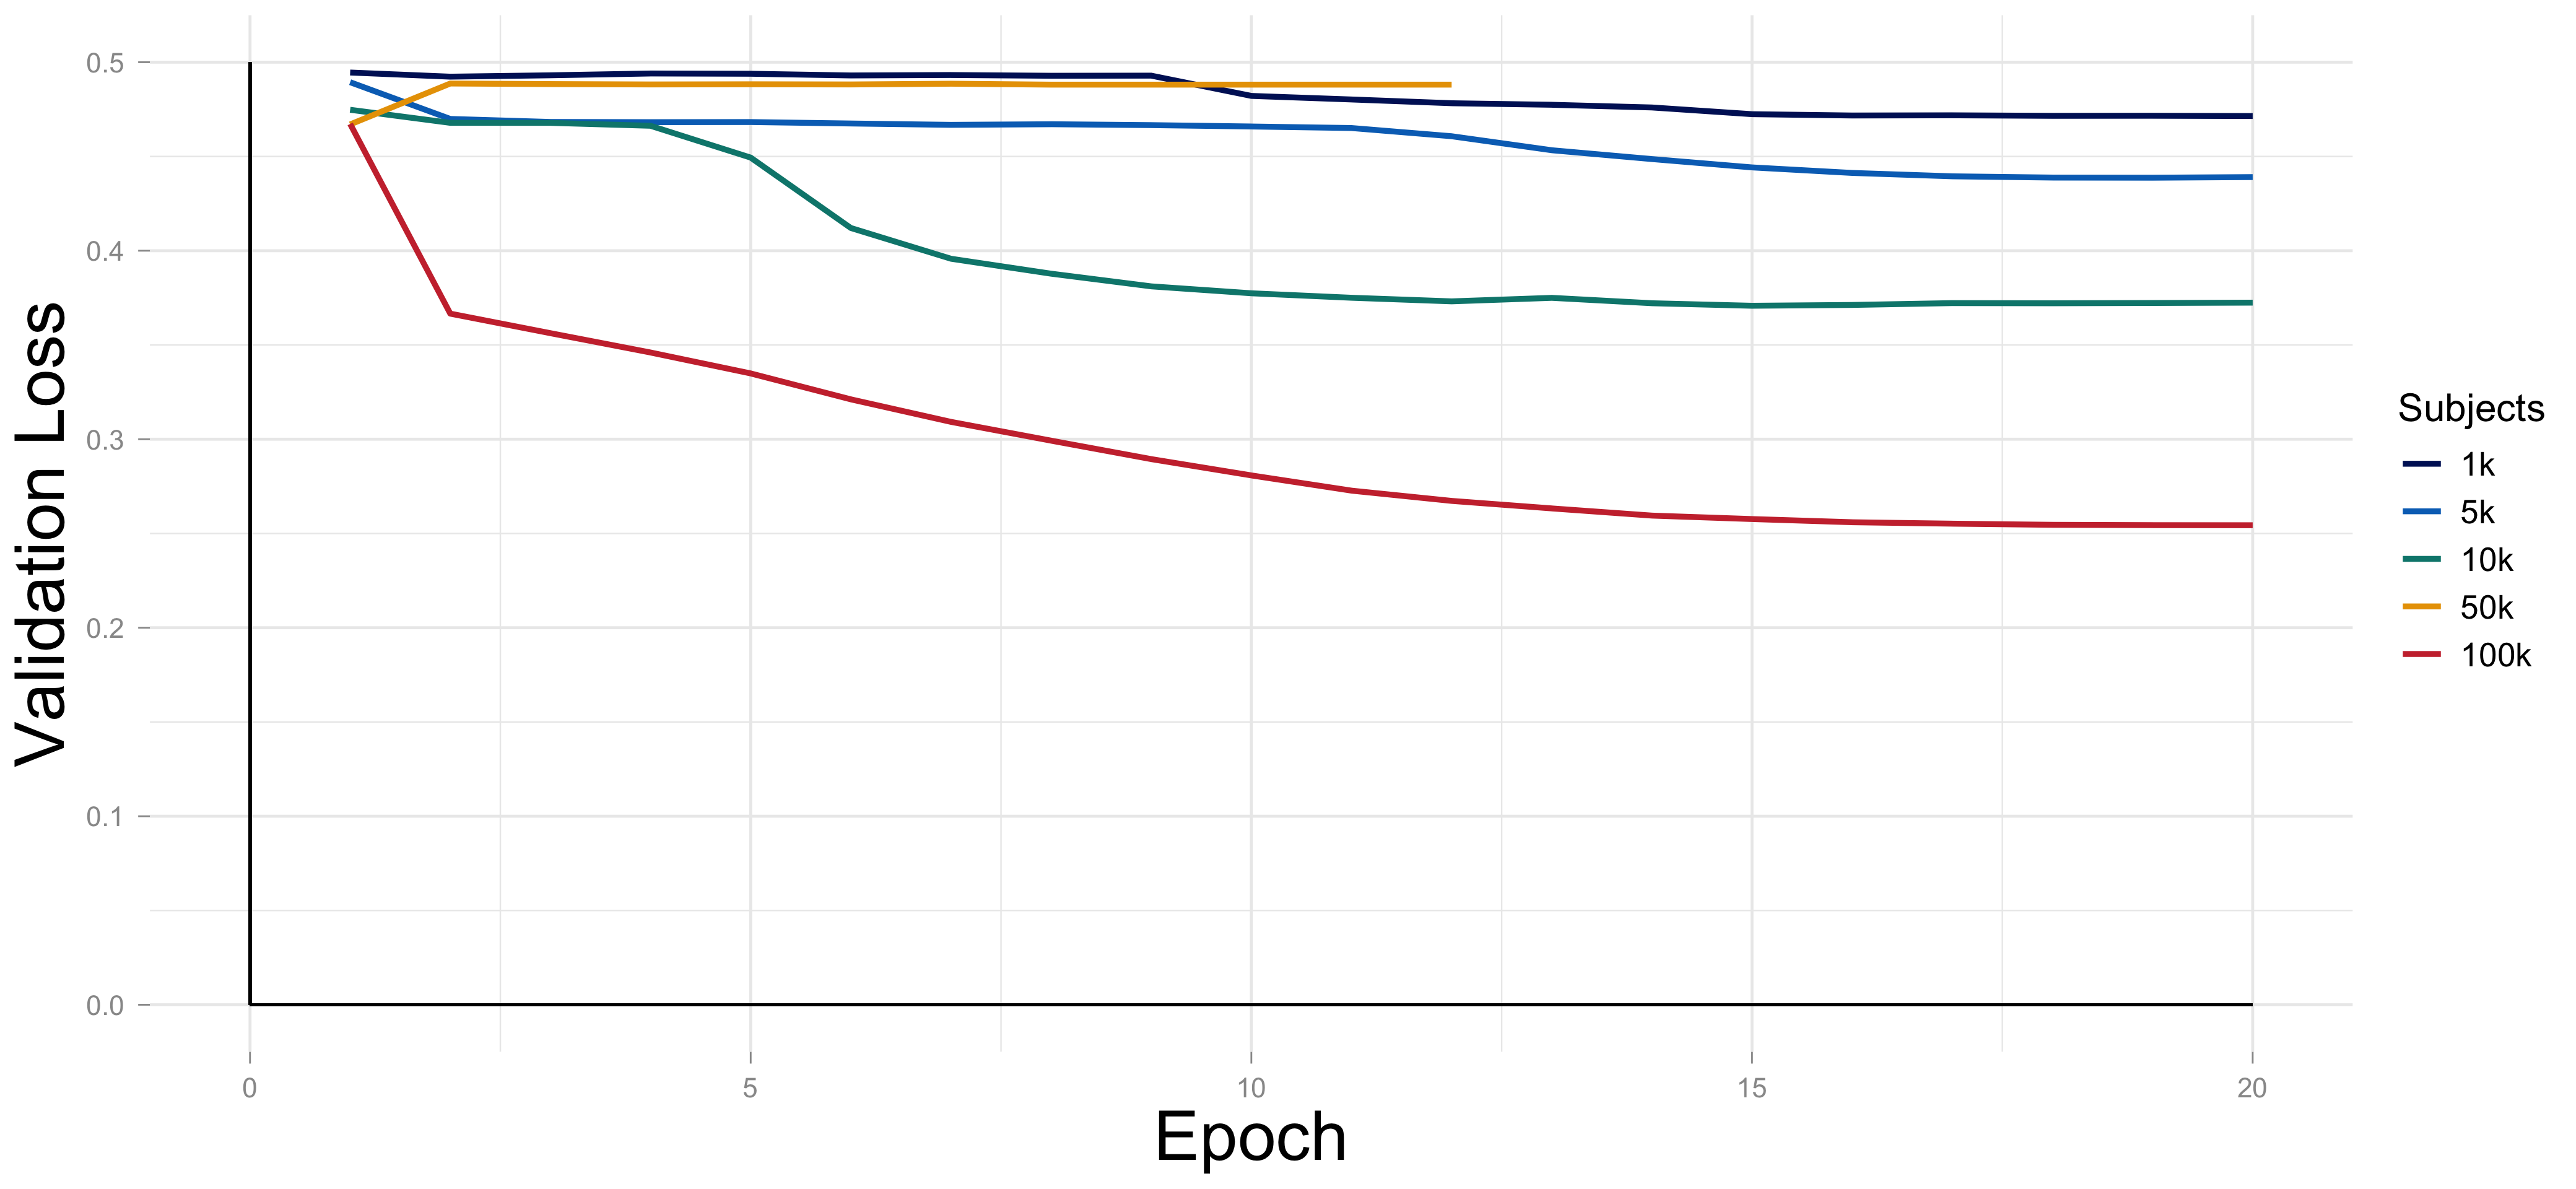
\includegraphics[width=0.95\linewidth]{fig/img/Pretrain/ValLoss.png}
    \caption{Validation loss during pre-training of SNPbag across different training set sizes. Each curve shows the masked cross-entropy loss on the validation set as a function of epoch, for training sets of $1000$, $5000$, $10000$, $50000, \text{and } 100000$ individuals. All runs use $M = 14000$ SNPs from chromosome~22, a mask probability of $0.85$, and $20$ epochs.}
    \label{fig:pretrain_val_loss}
\end{figure}

 
After pre-training, the SNPbag encoder has learned contextualised representations of genotype sequences from the masked genotype modelling objective without any phenotype information. Fine-tuning adapts these representations for binary phenotype prediction by replacing the masked genotype prediction head with a phenotype prediction head, as described in \autoref{sec:php}.
 
\subsection{Model Construction}

The fine-tuning model is constructed by loading the pre-trained encoder parameters with the lowest validation loss from the $100000$-individual run as the starting point of the prediction model.. The encoder and embedding architecture is identical to the pre-training configuration described in \autoref{tab:pretrain_hyperparams}. The masked genotype prediction head is discarded and replaced by a phenotype head, as described in \autoref{sec:php}.

Since the phenotype is defined for an entire individual rather than per-SNP, the encoder outputs are aggregated by mean pooling into a single vector per individual, which is passed to the phenotype head to obtain a predicted logit, as described in \autoref{sec:php}.
 
\subsection{Training Procedure}
\label{sec:app_finetune}
 %Freeze the encoder
Fine-tuning uses the same $70$/$10$/$20$ data split as LDpred2-auto, ensuring both methods are evaluated on identical individuals.
 
Due to a limited computational budget, the pre-trained encoder parameters are frozen during fine-tuning. This means that only the phenotype head is trained, while the encoder and embedding weights remain fixed at the values learned during pre-training. Freezing the encoder substantially decreases both the memory footprint and the time required per training step. The trade-off is that the encoder cannot adapt its representations to the phenotype prediction task, so the model relies entirely on the genomic context already captured during masked genotype pre-training.

Training was done for a single epoch with batch size $144$, distributed across $8$ GPUs, and the resulting model is evaluated on the test set using accuracy and AUC.

\section{Comparison of SNPbag and LDpred2-auto}
\label{sec:app_comparison}
 
Both methods are evaluated on the same test set $\mathcal{I}_{\text{test}}$ of $20000$ individuals using two metrics: classification accuracy at a threshold tuned on the validation set, and the area under the receiver operating characteristic curve (AUC). The results are summarised in \autoref{tab:comparison} and the ROC curves are shown in \autoref{fig:roc_comparison}.
 
\begin{table}[H]
\centering
\caption{Test set performance of LDpred2-auto and SNPbag on the simulated binary phenotype. The phenotype is simulated with the logistic disease model \citep{Majumdar2018} with $|\mathcal{M}_c| = 500$ causal SNPs, $\sigma_\beta = 0.5$, and a target prevalence of $K = 0.10$. Both methods are trained on $70\,000$ individuals, validated on $10\,000$ individuals, and tested on $20\,000$ individuals.}
\label{tab:comparison}
\begin{tabular}{l c c}
\toprule
\textbf{Method} & \textbf{Accuracy} & \textbf{AUC} \\
\midrule
LDpred2-auto & \texttt{0.507} & \texttt{0.510} \\
SNPbag       & \texttt{0.529} & \texttt{0.540} \\
\bottomrule
\end{tabular}
\end{table}

\begin{figure}[h]
    \centering
    \begin{subfigure}[t]{0.48\linewidth}
        \centering
        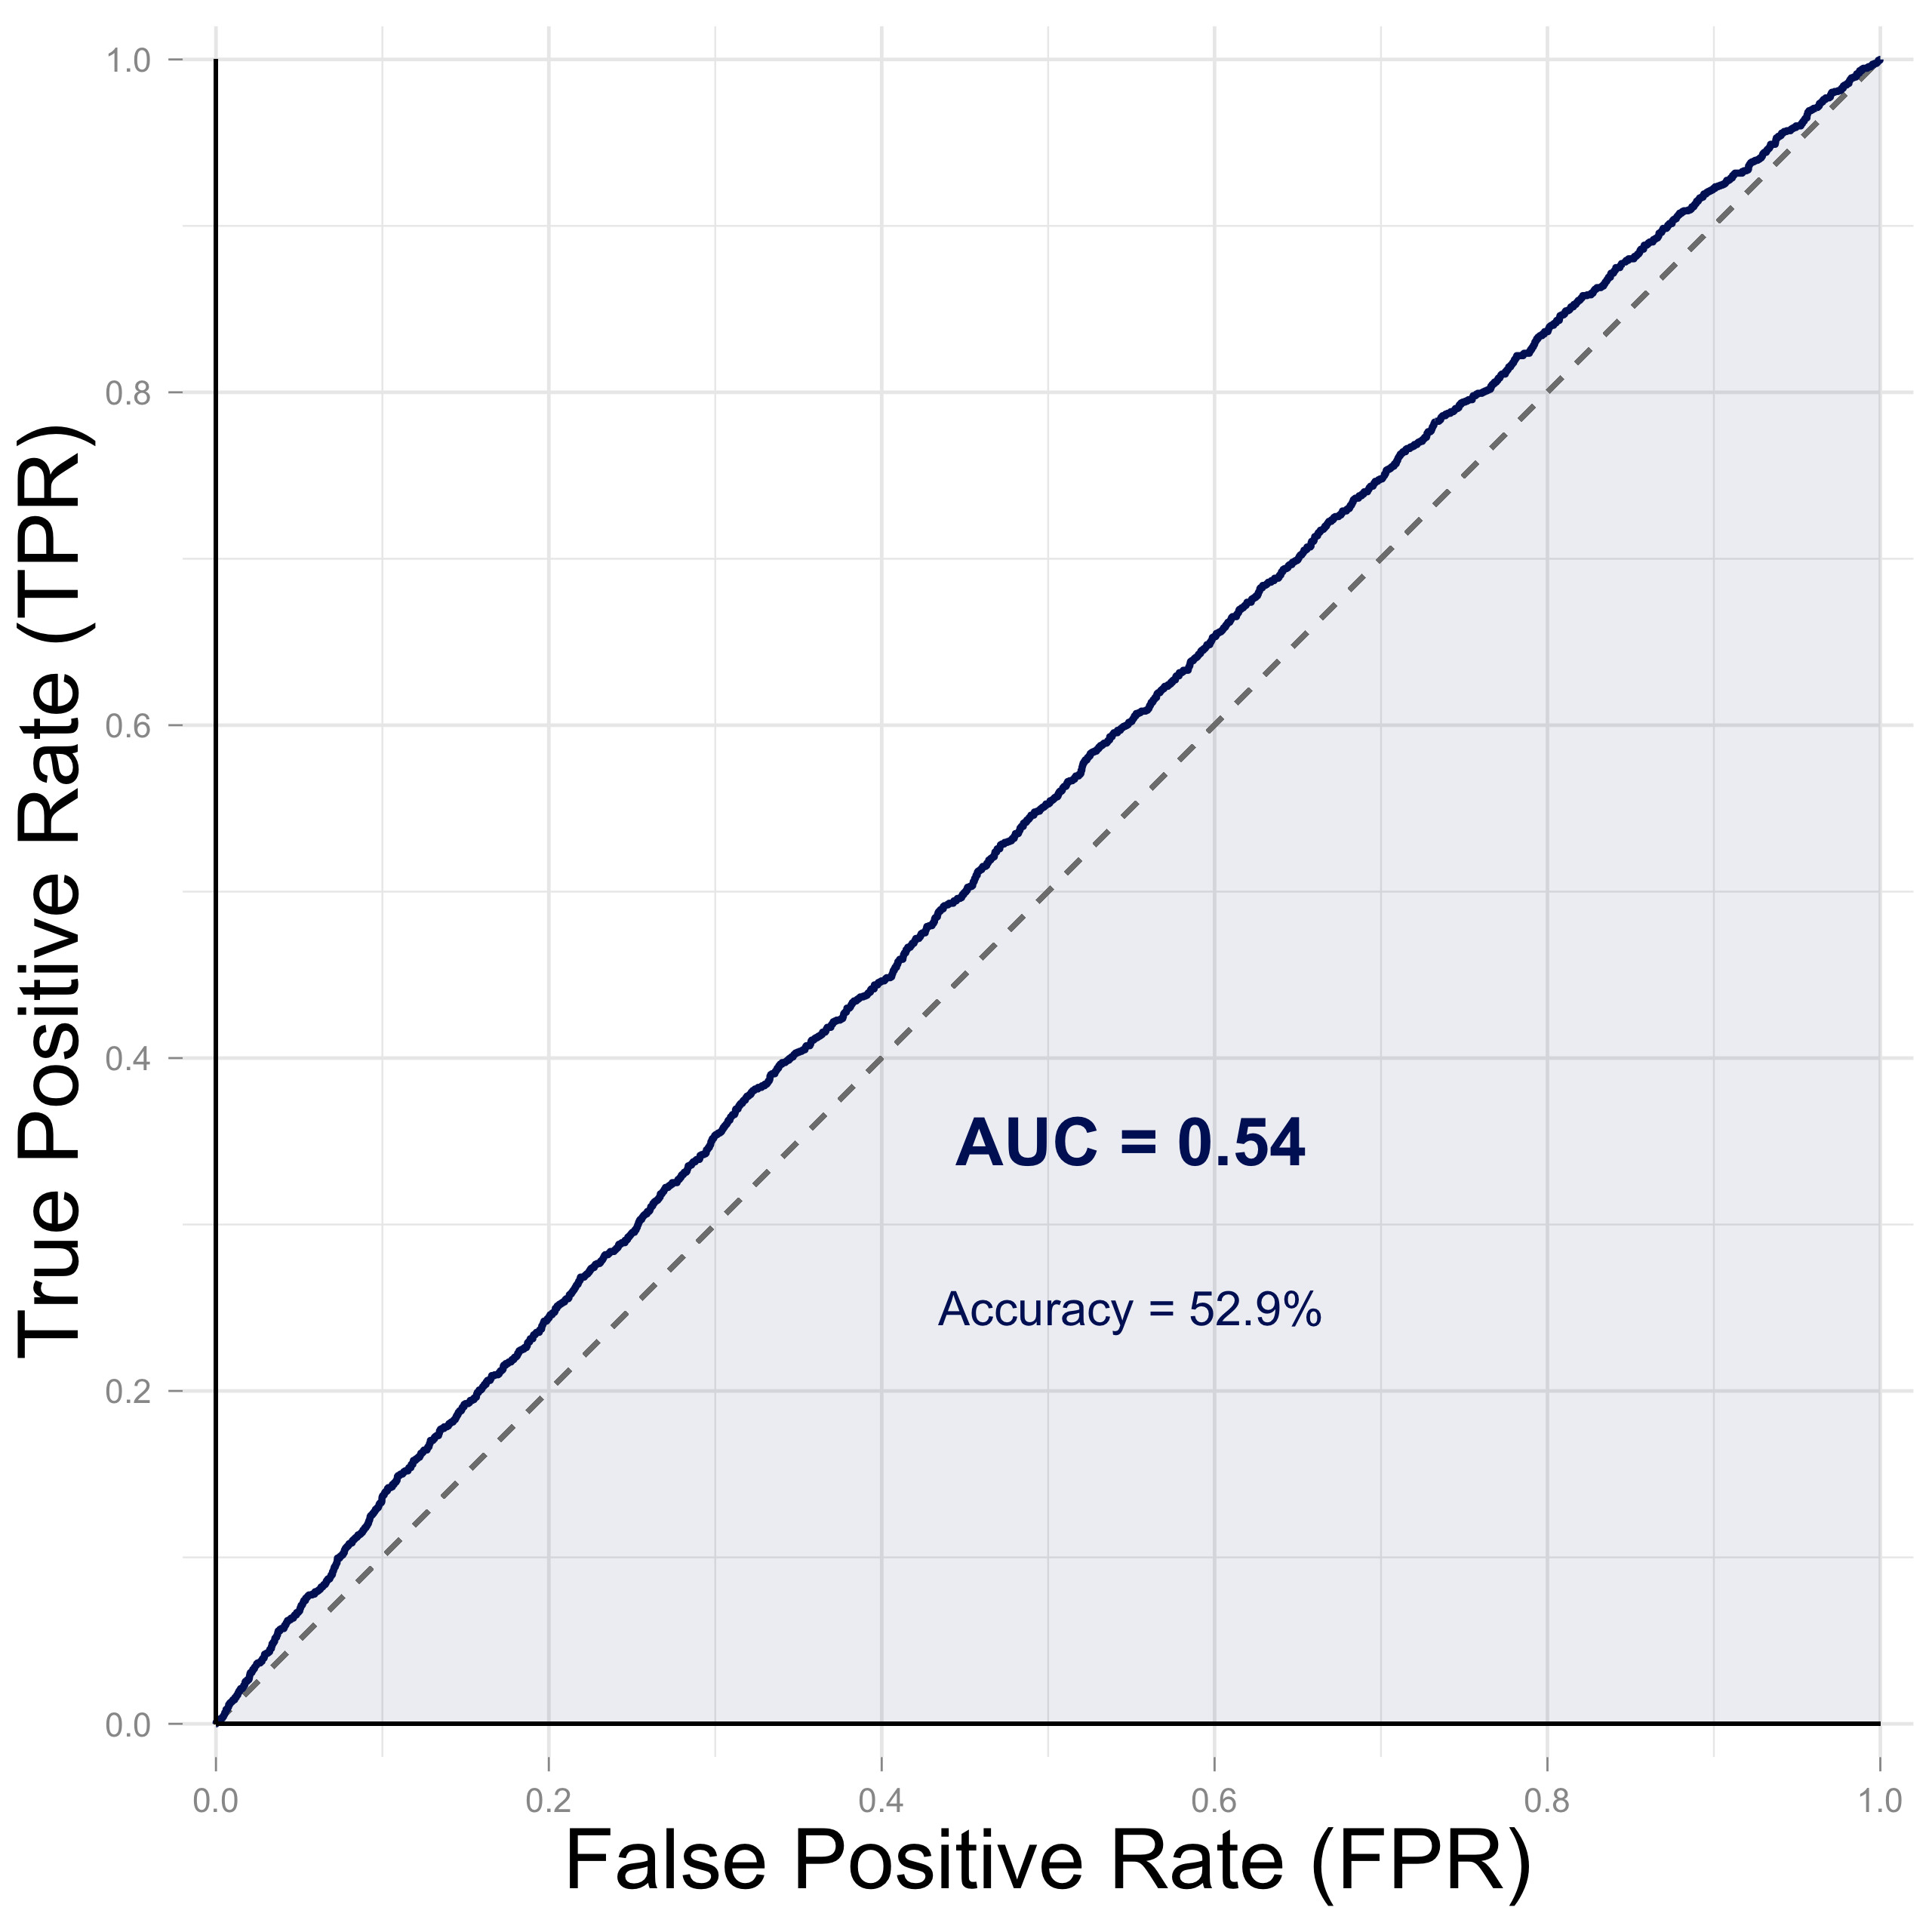
\includegraphics[width=\linewidth]{fig/img/SimStudy/ROC_SNPbag.png}
        \caption{SNPbag ($\mathrm{AUC} = 0.54$).}
        \label{fig:roc_snpbag}
    \end{subfigure}
    \hfill
    \begin{subfigure}[t]{0.48\linewidth}
        \centering
        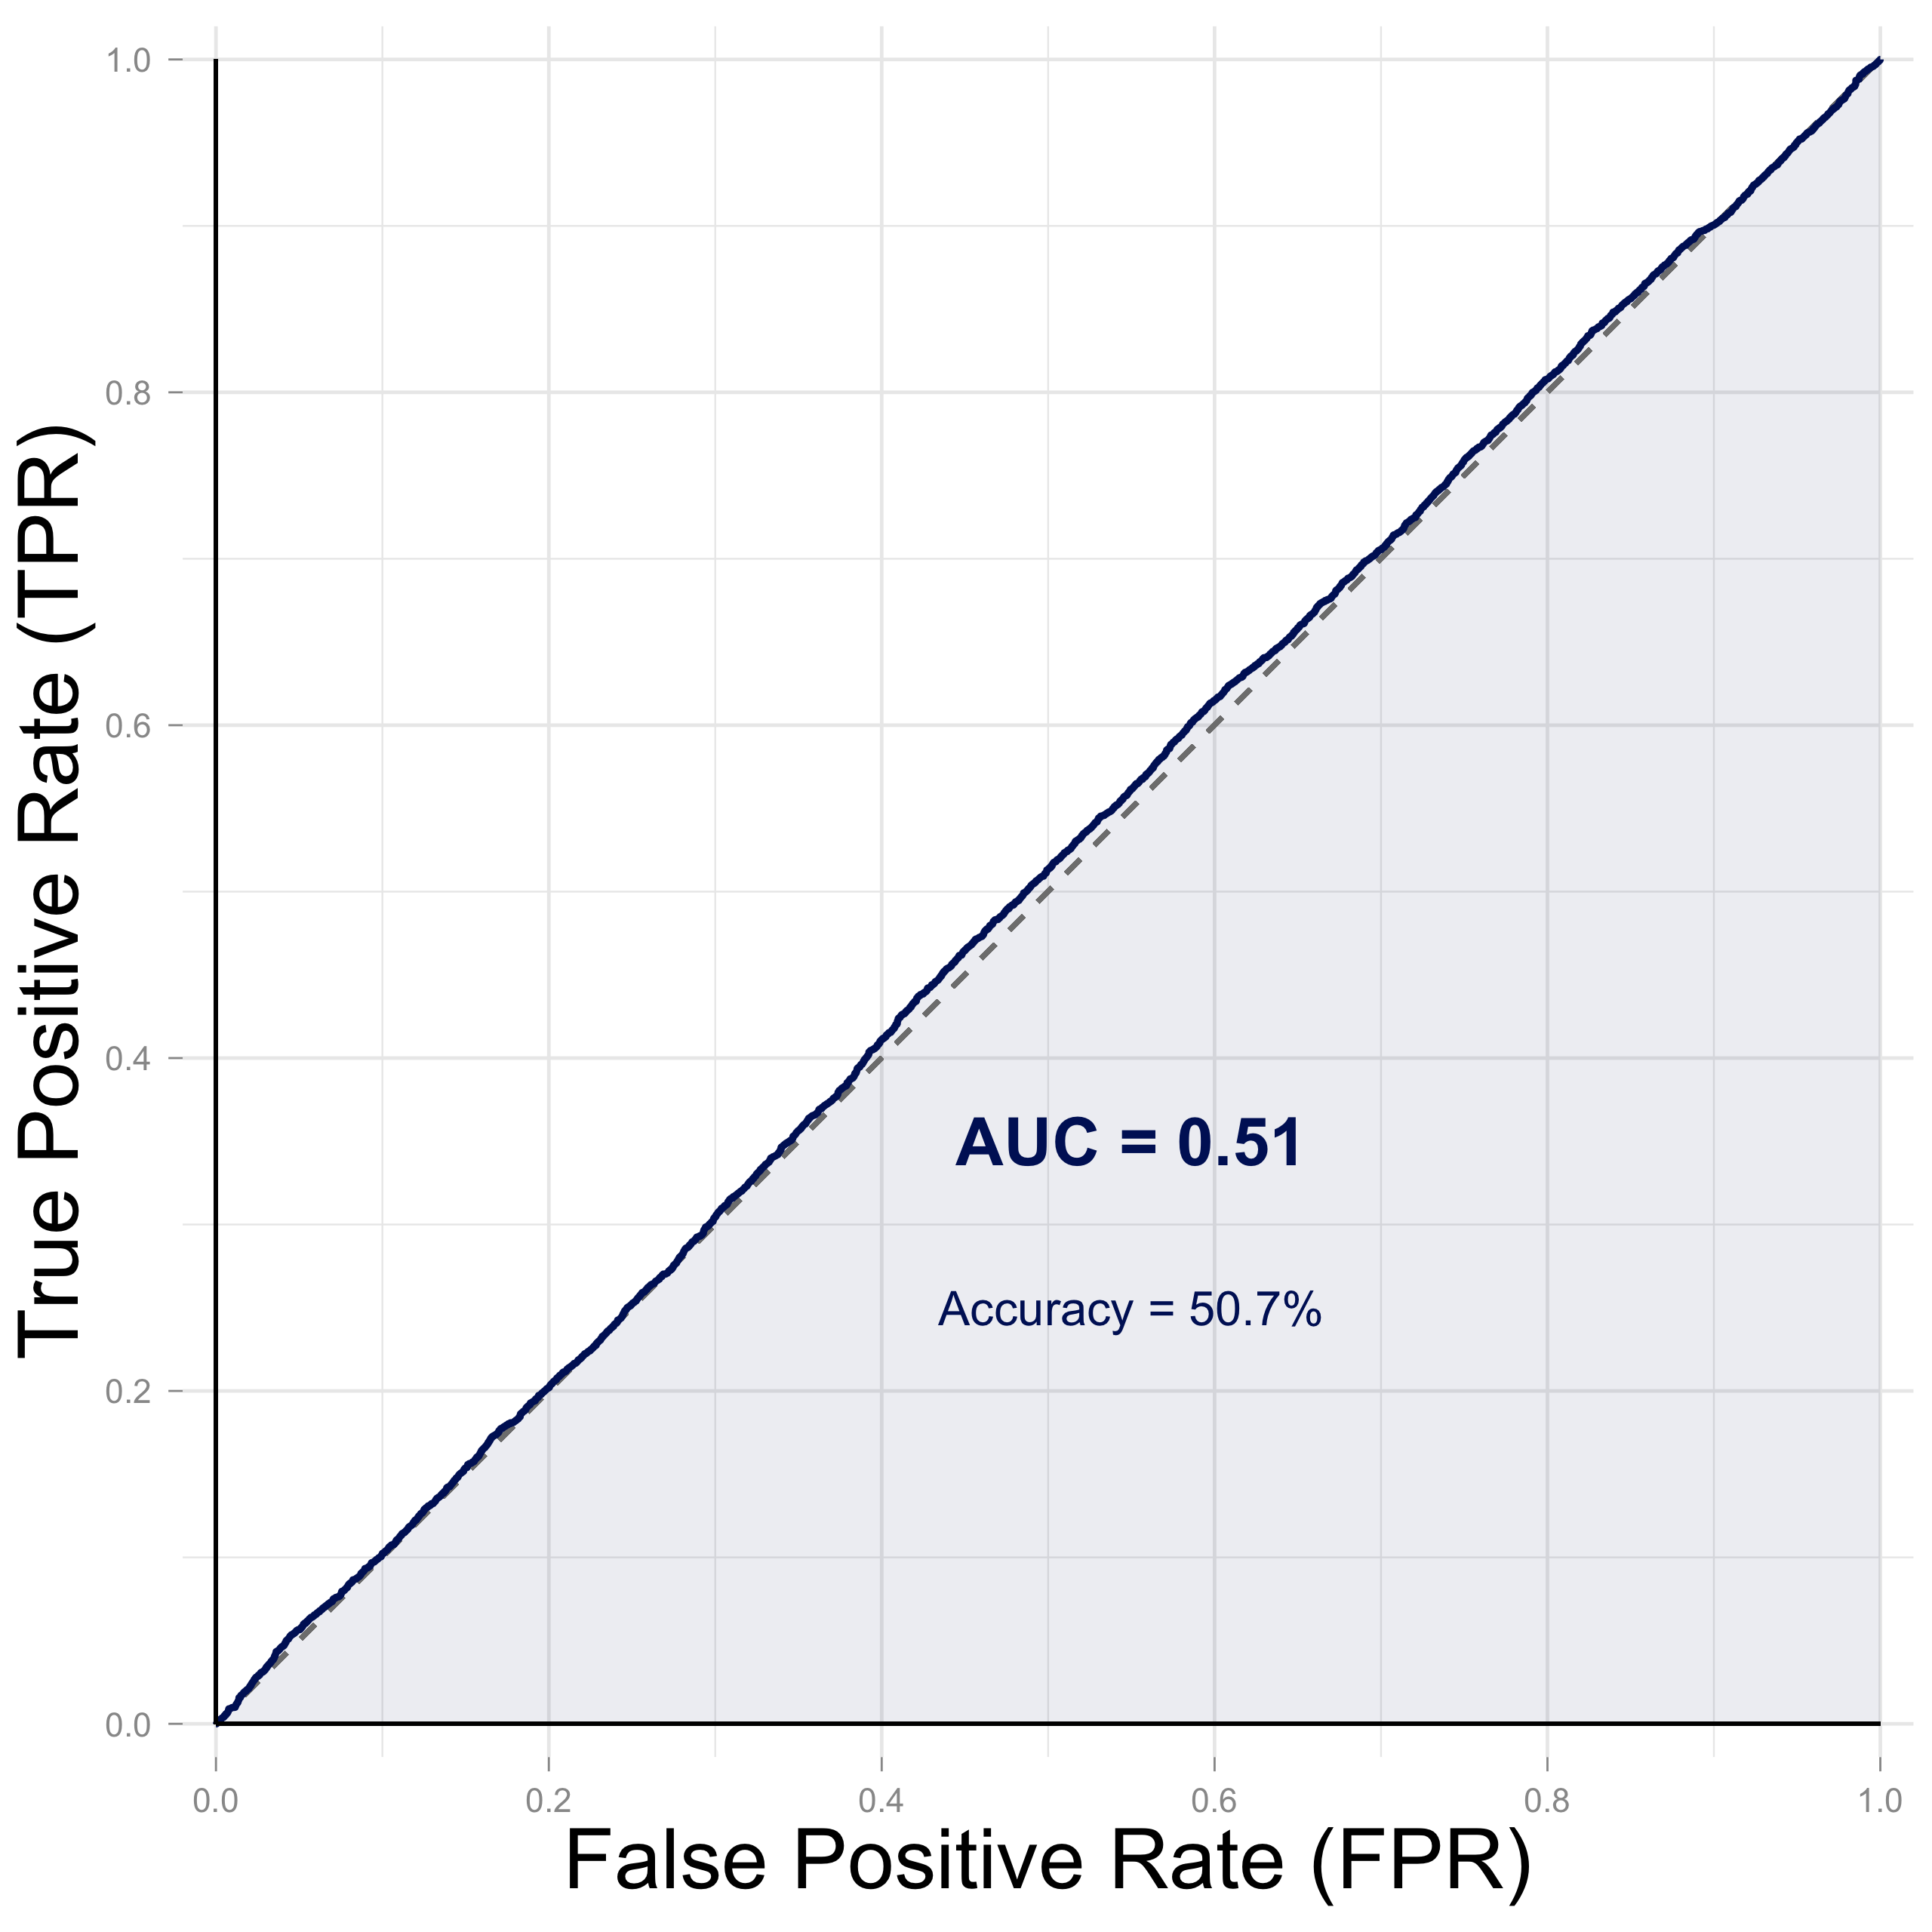
\includegraphics[width=\linewidth]{fig/img/SimStudy/ROC_GLM_LDpred2.png}
        \caption{LDpred2-auto ($\mathrm{AUC} = 0.51$).}
        \label{fig:roc_ldpred2}
    \end{subfigure}
    \caption{ROC curves on the test set for SNPbag and LDpred2-auto on the simulated binary phenotype described in \autoref{tab:comparison}. The shaded area corresponds to the AUC, and the dashed line represents a random classifier ($\mathrm{AUC} = 0.5$). Both curves lie close to the diagonal, indicating that neither method achieves meaningful discriminative power in this setting.}
    \label{fig:roc_comparison}
\end{figure}

The SNPbag achieved an accuracy of $52.9\%$, with an AUC of $0.54$, only slightly above the random baseline of $0.5$, which confirms that the model has minimal discriminative power. LDpred2-auto similarly shows a near-random AUC of $0.51$. Neither method achieved meaningful phenotype prediction in this setting. This is likely due to a combination of factors: SNPbag was limited to a single epoch with a frozen encoder, LDpred2-auto operated on only $14000$ SNPs from a single chromosome, and genotype-based prediction can at most explain the heritability $h^2$ of the trait, meaning that a substantial fraction of the phenotypic variation is driven by environmental factors that no genotype model can capture.